\documentclass[11pt]{article}
\usepackage{amsmath, amssymb}
\usepackage{geometry}
\geometry{margin=1in}
\usepackage{fancyhdr}
\usepackage{lastpage}
\usepackage{parskip} % Better paragraph spacing
\usepackage{titlesec} % Better section formatting
\usepackage{graphicx}
\usepackage{float}
\usepackage[most]{tcolorbox}
\usepackage{lmodern}
\usepackage{caption}
\usepackage{hyperref}
\usepackage{multicol}

% Define commands for reusable content
\newcommand{\coursename}{COM-407 Advanced Networks}
\newcommand{\lecturenum}{10}
\newcommand{\lecturedate}{\today}
\newcommand{\professor}{Pavlos Nikoupoulos}

\hypersetup{colorlinks=true,linkcolor=blue,urlcolor=blue}

% Configure section spacing
\titlespacing*{\section}{0pt}{2ex plus 1ex minus .2ex}{1.5ex plus .2ex}
\titlespacing*{\subsection}{0pt}{1.5ex plus 1ex minus .2ex}{1ex plus .2ex}
% Header / Footer
\pagestyle{fancy}
\fancyhf{}
\fancyhead[L]{\coursename}
\fancyhead[R]{Lecture \lecturenum}
\fancyfoot[L]{EPFL - Computer Science}
\fancyfoot[C]{Author: Jonathan Dutoit}
\fancyfoot[R]{Page \thepage\ of \pageref{LastPage}}

\begin{document}

\begin{center}
  {\large EPFL - Computer Science} \\[0.5em]
  {\Large \textbf{\coursename}} \\[0.5em]
  {\large Lecture \lecturenum\ --- \lecturedate} \\[0.5em]
  {\large Author: Jonathan Dutoit} \\[0.5em]
  {\large Professor: \professor} \\[0.5em]
\end{center}

\vspace{2cm}

\begin{center}
  {\LARGE \textbf{Routing Algorithms (Part 2)}}
\end{center}

\vspace{1cm}

\section*{5. OSPF's reactions to changes in topology}

Changes occur when links or routers fail or reboot

The routes detect failures via:
\begin{itemize}
	\item OSPF's hello protocol (after several seconds, in general)
	\item Bidirectional Forwarding Detection (BFD) protocol: hello protocol at the Ethernet layer (fast: after 10ms, independent of OSPF)
	\item directly - no power on the cable
\end{itemize}

Upon a detected failure/change:
\begin{itemize}
	\item router floods \textcolor{blue}{\textit{new LSA}} with new sequence number and \textcolor{blue}{\textit{new (alive)}} neighbors
	\item neighbors propagate new LSA
	\item all routers update their LSDB, re-compute shortest paths and forwarding tables
\end{itemize}

Problems: while fixing failures, it takes \textcolor{red}{time} and may result in \textcolor{red}{transient routing loops} and packet \textcolor{red}{drops}

\subsection*{Example of changes in the topology}

% Quick centered image
\begin{figure}[H]
    \centering
    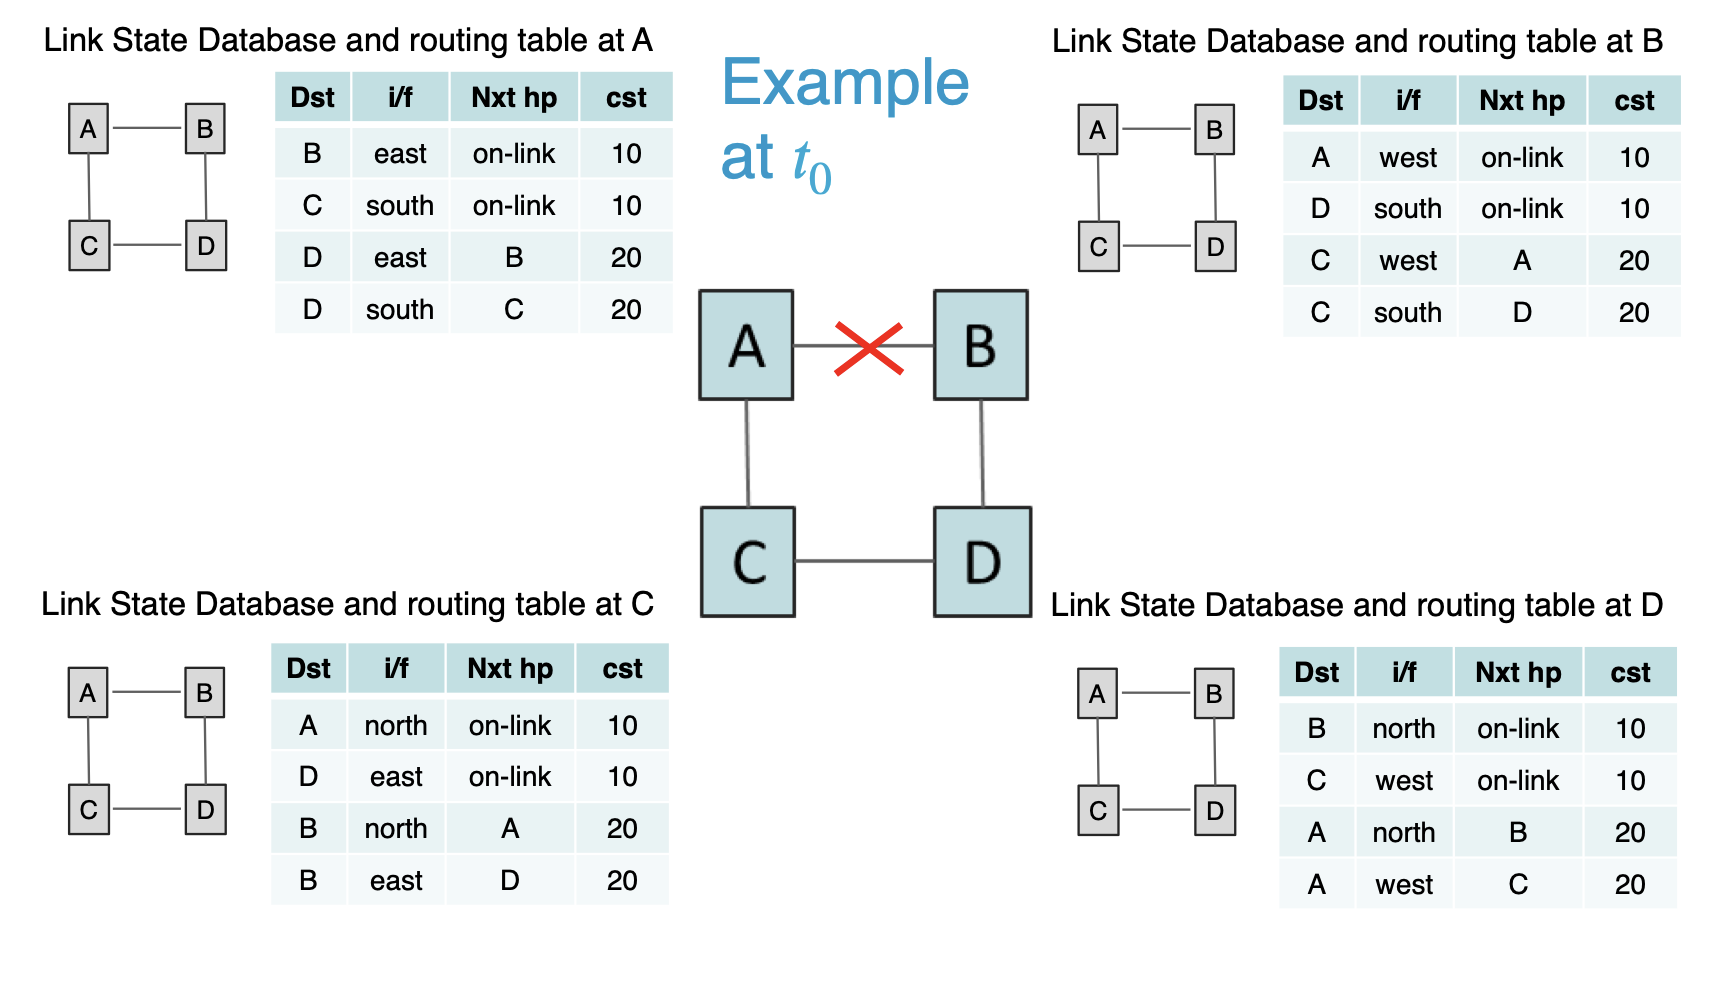
\includegraphics[width=0.8\textwidth]{images/link-crash}
    \label{fig:LABEL}
\end{figure}
\begin{itemize}
	\item $t_0$: Link A-B crashes
	\item $t_1$: A detects failure first; declares B as invalid neighbor, declares link A-B as invalid, sends a new LSA to C, with origin A and recomputes its forwarding table.
	\item A \textcolor{red}{\textit{transient routing loop}} is created between A and C for destination B. Traffic sent by B to A dies on the link, until B detects the failure. So, half of the traffic from D to A is also lost. Analogy for Internet Protocol Layer is TTL to avoid loops.
	\item $t_2$: C receives LSA from A, updates its LSDB, forwards this LSA to D and recomputes forwarding table. B hasn't detected the failure yet. There is no routing loop but traffic sent by B to A dies on the link and half of the traffic from D to A is lost.
	\item $t_3$:  D receives LSA from C, updates its LSDB, forwards this LSA to B and recomputes forwarding table.
At about the same time, B also detects failure; declares A as invalid neighbor, declares link A-B as invalid, updates its
LSDB, sends a new LSA to D, with origin B and recomputes routing table.
\end{itemize}

All LSDBs now have the same contents and new routes are in place.

\begin{tcolorbox}[
  colback=gray!15,     % background color
  colframe=black!50,    % border color
  boxrule=1pt,       % border thickness
  arc=3mm,             % rounded corners
  left=4mm, right=4mm, top=2mm, bottom=2mm % padding
]
\textbf{When a router crashes, how do other \textbf{remote} routers in area detect the crash?}

\vspace{0.3cm}

A. By a newly flooded LSAs: the immediate neighbors detect loss of adjacency and flood new LSAs with the updated list of adjacent/neighbor routers \\
B. By the hello protocol \\
C. By timeout of LSAs stored in their link-state database \\
D. By absence of BFD messages \\
E. I don't know \\

\textbf{Answer:} A (in principle) \\
Answer C is some rare cases possible, but normally neighbors detect the failure well before the LSA ages out (1 hour by default) \\

With the hello protocol and BFD, \textcolor{red}{only immediate neighbors} can detect the crashed router
\end{tcolorbox}

\section*{6. OSPF: Security aspects}

Attacks against routing protocols:

(1) send \textcolor{red}{invalid} routing information: \textcolor{red}{disrupt} network operation \\
(2) send \textcolor{red}{forged} routing information: \textcolor{red}{change} network paths \\
(3) denial of service attacks \\

OSPF \textcolor{blue}{\textit{authentication}} mitigates (1) and (2)

OSPFv3 uses IPSEC authentication

We use symmetric key because network administrator can pre-install them in routers. Asymmetric cryptography is too expensive since we need to transmite LSAs to all nodes of the network constantly. 

% Quick centered image
\begin{figure}[H]
    \centering
    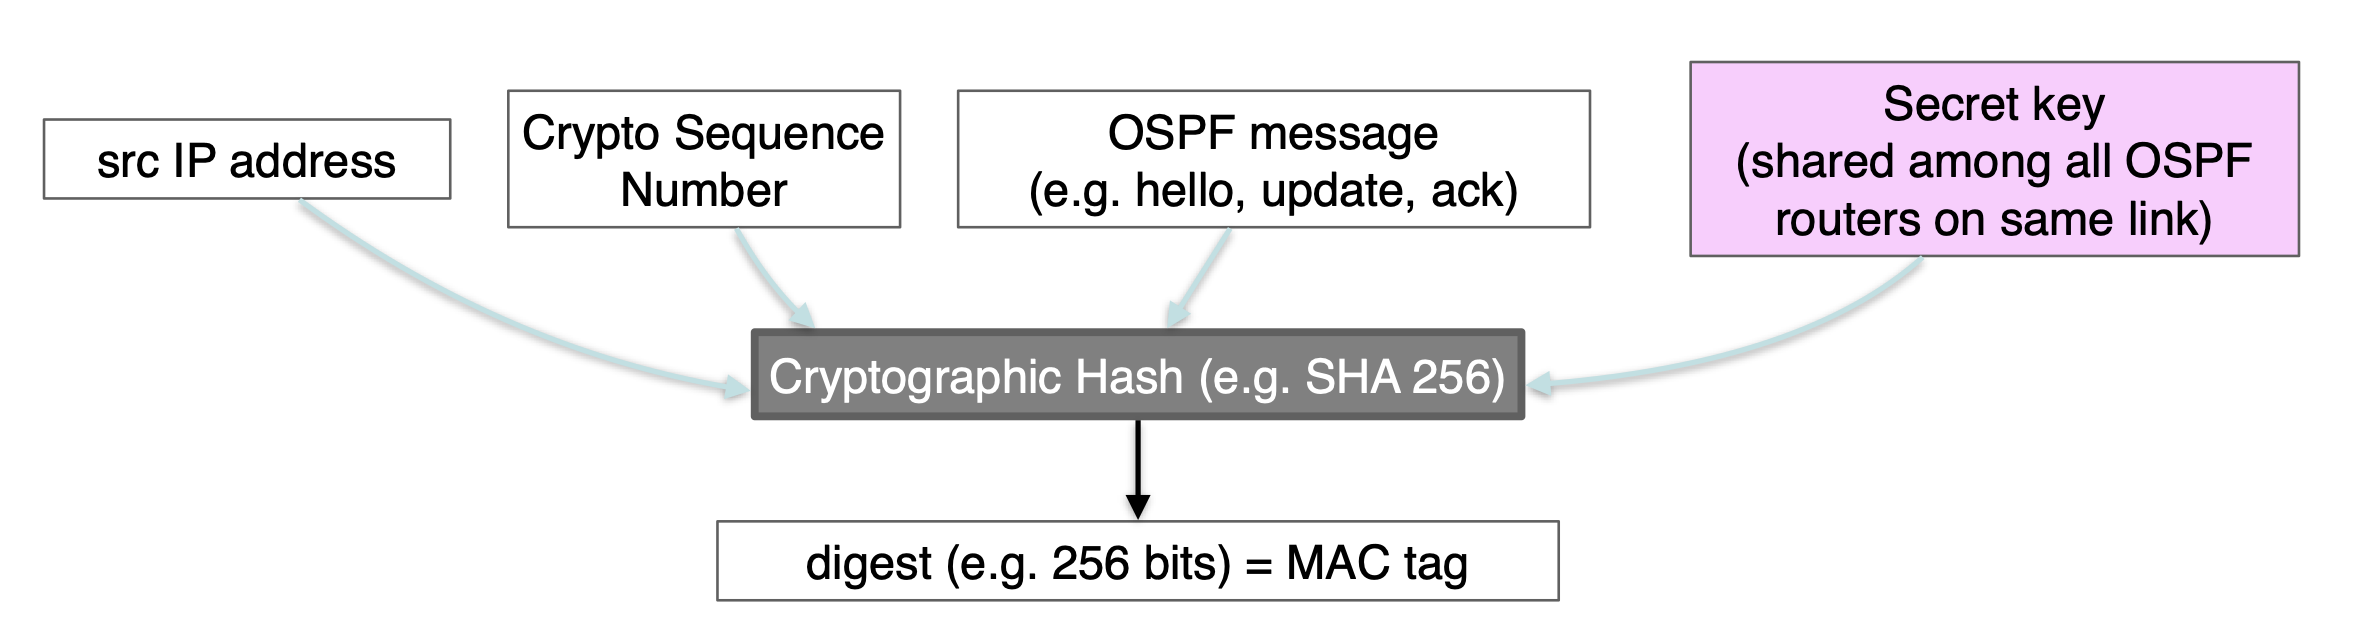
\includegraphics[width=0.8\textwidth]{images/ospf-auth}
    \label{fig:LABEL}
\end{figure}
\begin{itemize}
	\item Digest is appended to OSPF message, and is used as \textcolor{red}{\textit{message authentication code (MAC tag)}}
	\item Secret key is shared and has a short lifetime:
	\begin{itemize}
		\item Neighbors have pre-installed the same list of keys (installation via an \textbf{\textit{out-of-band}} mechanism)
		\item A key index in the authentication header of an OSPF message points to the used key
	\end{itemize}
	\item Crypto Sequence Number avoids \textcolor{red}{\textit{replay attacks}}
		\begin{itemize}
			\item 64-bit number incremented for every OSPF packet; numbers never wrap around
			\item First 32 bits are "boot count" saved on hard disk to avoid collision of numbers after reboot
			\item The number is also added to OSPF authentication header in cleartext (for the neighbor to verify the MAC tag)
		\end{itemize}
\end{itemize}

\section*{7. OSPF with Multiple Areas}

\textcolor{red}{Why?} LSA flooding does \textcolor{red}{\textit{not scale}} in very large networks

OSPF uses \textcolor{blue}{\textit{multiple}} areas and a 2-level \textcolor{blue}{\textit{hierarchy}}
\begin{itemize}
	\item a \textcolor{red}{\textit{backbone area}} (area 0)
	\item several non-backbone areas
\end{itemize}

All inter-traffic goes through backbone area 0

% Quick centered image
\begin{figure}[H]
    \centering
    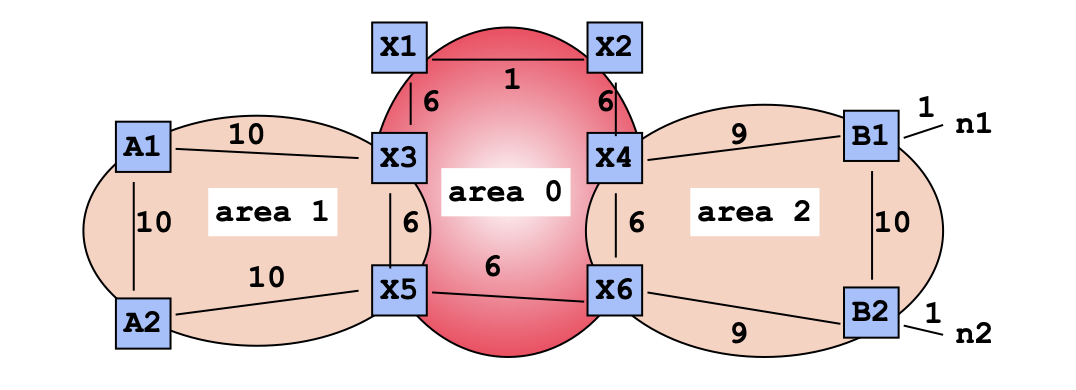
\includegraphics[width=0.6\textwidth]{images/ospf-backbone}
    \label{fig:LABEL}
\end{figure}

\subsection*{Principles of OSPF Multi-Area Operations}
1. Within an area use classic link state - single LSDS per area (for all routers in area) 

2. Between areas, use \textcolor{red}{\textit{border routers}}:
\begin{itemize}
	\item belong to both areas and have 2 LSDBs
	\item inject \textcolor{red}{\textit{aggregated distance (cost) information}} learnt from one area into the other area by using \textcolor{blue}{\textit{summary LSAs}}
\end{itemize}

\newpage

\subsection*{Example}

% Quick centered image
\begin{figure}[H]
    \centering
    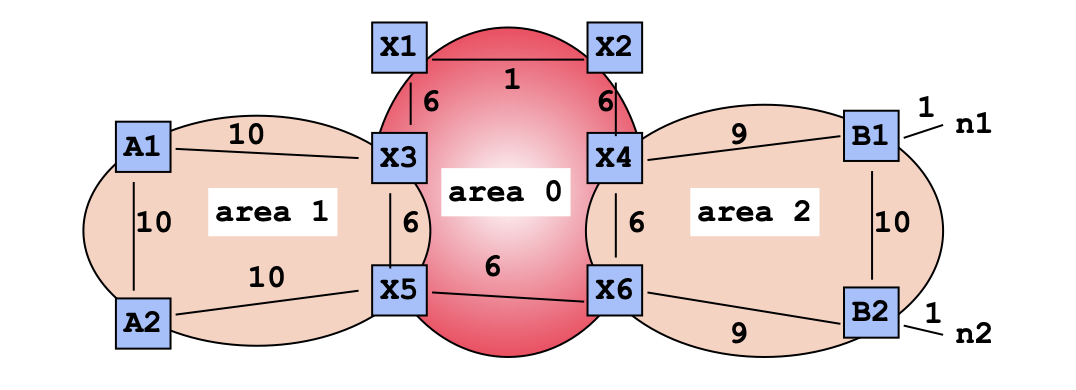
\includegraphics[width=0.6\textwidth]{images/ospf-backbone}
    \label{fig:LABEL}
\end{figure}

\begin{multicols}{3}

\section{Step}
\begin{itemize}
	\item All routers in area 2 flood the LSAs originated by B1 and B2 and know of n1 and n2, directly attached to B1 (resp. B2). This is the normal link state operation.
	\item All routers in area 2 have the same link state database
	\item All routers in area 2, including X4 and X6 compute their distances to n1 and n2 (using Dijkstra)
\end{itemize}

\section{Step}
\begin{itemize}
	\item X4 and X6 each flood into area 0 a \textcolor{red}{\textit{summary LSA}} indicating their distances to n1 and n2.
	\item All routers in area 0 now have the same link database.
	\item All routers in area 0, including X3 and X5 computer their distances to networks onside the area (such as n1) using the Bellman-Ford formula:
		\[
			d(self, n1) =\\ \underset{BR \in Area0}{\min} \{ d(self, BR) + d(BR, n1)\}
		.\] 

\end{itemize}

\section{Step}
\begin{itemize}
	\item X3 and X5 each flood into Area 1 a \textcolor{red}{\textit{summary LSA}} indicating their distances to n1 and n2.
	\item All routers in Area 1 now have the same link database.
	\item All routers in Area 1 compute their distances to networks outside the area (such as n1) using a similar Bellman-Ford formula. 
\end{itemize}
\end{multicols}


\begin{tcolorbox}[
  colback=gray!15,     % background color
  colframe=black!50,    % border color
  boxrule=1pt,       % border thickness
  arc=3mm,             % rounded corners
  left=4mm, right=4mm, top=2mm, bottom=2mm % padding
]
\textbf{When applying the Bellman-Ford formula to compute $d(self, n1)$, how does a router such as A1 know the values of  $d(self, BR)$ and  $d(BR, n1)$}

\vspace{0.3cm}

A. $d(self, BR)$ from its routing table after applying Dijkstra and  $d(BR, n1)$ from the summary LSA received \\
B.  $d(BR, n1)$ from its routing table after applying Dijkstra and  $d(self, BR)$ from the summary LSA received \\
C. Both from its routing table after applying Dijkstra \\
D. Both from the summary LSA \\
E. I don't know \\

 \textbf{Answer:} A.  \\

 All routers in area 1 have only their routing tables from step 1. The border routers are in area 1, so A1 knows $d(self, BR)$ from its routing table after applying Dijkstra and  $d(BR, n1)$ is know from a summary-LSA. 
\end{tcolorbox}

\begin{tcolorbox}[
  colback=gray!15,     % background color
  colframe=black!50,    % border color
  boxrule=1pt,       % border thickness
  arc=3mm,             % rounded corners
  left=4mm, right=4mm, top=2mm, bottom=2mm % padding
]
\textbf{How many link state database does router X3 have?}

% Quick centered image
\begin{figure}[H]
    \centering
    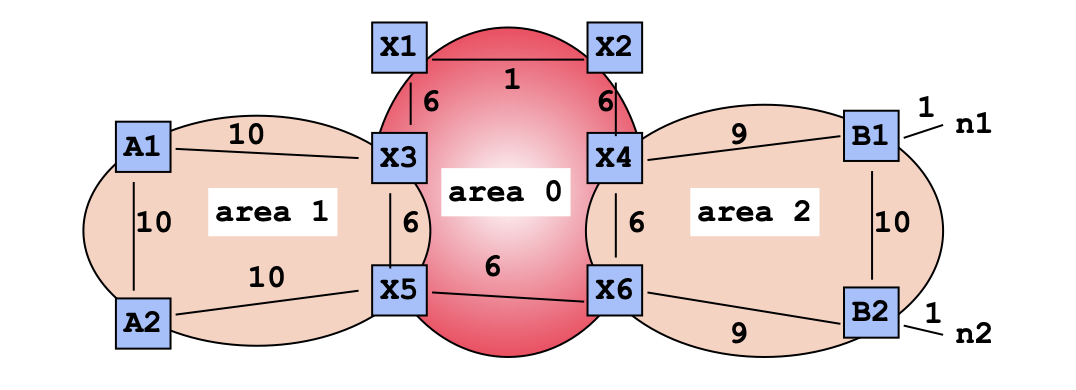
\includegraphics[width=0.6\textwidth]{images/ospf-backbone}
    \label{fig:LABEL}
\end{figure}
\vspace{0.3cm}

A. 1 \\
B. 2 \\
C. 3 \\
D. 0 \\
E. I don't know \\

\textbf{Answer}: B (2). X3 belongs to area 0 and to area 1 (border router). It has one link-state database for each. 
\end{tcolorbox}
\section*{8. Other Uses of LSAs}

With LSAs, routers have a "\textcolor{blue}{complete network view}" (e.g., topology, costs, latencies, attached subnets, etc.)

This info can be used by other network functions:
\begin{itemize}
	\item \textcolor{red}{source routing}: an edge router computes the entire path (not only next-hop), then writes it in an extension packet header. Avoids transient loops / supports fast re-route after failure. Used in deterministic networks (industrial applications)
	\item \textcolor{red}{multi-class routing}: compute different routes for different types of services (e.g., voice, video) based on different objectives (e.g., cost vs latency). Use the ""differentiated-services" field in IP header to forward traffic
	\item \textcolor{red}{LS bridging (VLAN-bridging via LS shortest paths}: connect different layer-2 VLANs \textit{over IP} instead of trunk cables
\end{itemize}

\subsection*{LS Bridging}
You want to bridge VLANs across a campus \textcolor{red}{\textit{without direct cables}}.

A solution: user routers that also implement a layer-2 switch, and \textcolor{purple}{\textit{tunnel}} (encapsulate) MAC packets in IP (which are also encapsulated in MAC)

Problem: automatic creation of tunnels.

\begin{tcolorbox}[
  colback=gray!15,     % background color
  colframe=black!50,    % border color
  boxrule=1pt,       % border thickness
  arc=3mm,             % rounded corners
  left=4mm, right=4mm, top=2mm, bottom=2mm % padding
]
\textbf{Can you imagine a solution using Link State Routing in R1, R2, ...}

\vspace{0.3cm}

A. Routers R1, R2,... discover which VLAN is active on any of their ports and put this information in the link state database \\
B. Routers R1, R2,... overhear all MAC source addresses and put the information in the link state database \\
C. Both of these solutions seem bad to me \\
D. I don't know \\

\textbf{Answer:} A. \\
B does not help since MAC addresses don't say in which VLAN the ,achine is. Recall that even with VLAN truck ports we needed the VLAN tag (= info about which VLAN a machine belongs to).
\end{tcolorbox}
\textbf{Exam question:} how to create a VLAN between a building at EPFL and some other place. This was asked in the exam last year


\begin{tcolorbox}[
  colback=gray!15,     % background color
  colframe=black!50,    % border color
  boxrule=1pt,       % border thickness
  arc=3mm,             % rounded corners
  left=4mm, right=4mm, top=2mm, bottom=2mm % padding
]
\textbf{"LS bridging" vs "Classic switches running STP": What is the maximum value of $\lambda$ we can achieve in each use?}

% Quick centered image
\begin{figure}[H]
    \centering
    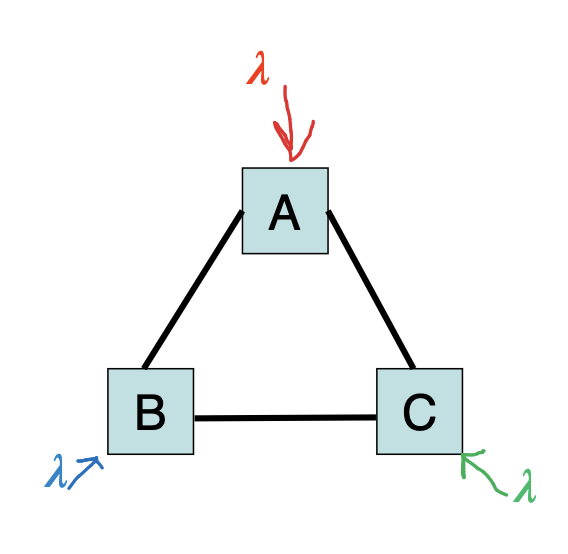
\includegraphics[width=0.25\textwidth]{images/ls-bridging-stp}
    \label{fig:LABEL}
\end{figure}

\begin{itemize}
	\item Node A want to send a total traffic rate equal to $\lambda$ b/s, half to B, half to C.
	\item Same for B and C
	\item Link capacities are 1 Gb/s in every direction (full duplex).
	\item OSPF costs are the \textit{same} everywhere.
	\item Possible configuration: OSPF Routers or Switches with STP.
\end{itemize}

\vspace{0.3cm}

A. With OSPF: $\lambda_{max} = 2$ Gb/s; with STP $\lambda_{max} = 2$ Gb/s; \\
B. With OSPF: $\lambda_{max} = 2$ Gb/s; with STP $\lambda_{max} = 1$ Gb/s; \\
C. With OSPF: $\lambda_{max} = 1$ Gb/s; with STP $\lambda_{max} = 2$ Gb/s; \\
D. With OSPF: $\lambda_{max} = 1$ Gb/s; with STP $\lambda_{max} = 1$ Gb/s; \\
E. I don't know \\

\textbf{Answer:} B. \\
OSPF routers use shortest paths. Traffic from any node uses the direct link. From A to B, the traffic flow is $\lambda/2$, same on every link and each direction. Thus,  $\lambda_{max} = 2$ Gb/s \\

With switches, a spanning tree is build and one of the links is disable. Total traffic on every link and every direction is  $\lambda$. Thus,  $\lambda_{max} = 1$ Gb/s
\end{tcolorbox}
\section*{9. Routing in Software Defined Networks (SDNs)}

\textcolor{red}{Why is exists?} In principle, routers compute best paths using a \textit{distributed algorithm}, populate their forwarding tables, and use dest IP address + longest prefix match to decide where to forward packets. 

Some networks want \textcolor{blue}{\textit{more control}}; e.g., handle mission-critical traffic with higher priority; ban non-HTTP traffic; send suspicious/DoS traffic to a scrubber for inspection

\textcolor{red}{\textit{Deep packet inspection (DPI)}}: routers look not only at IP headers, but also ports and payload $\Rightarrow$ classify traffic according to  \textit{more} fields

\textcolor{red}{\textit{Per-flow forwarding}}: when a packet is to be forwarded, the router:
\begin{itemize}
	\item looks for a match in a \textcolor{blue}{flow table = \{per-flow forwarding} rules with \textcolor{blue}{priorities}\}
	\item If several rules match, router follows the rule with \textcolor{purple}{highest priority}
	\item If no rule matches, it goes to the IP forwarding table and does longest prefix match
\end{itemize}

Same ideas can be used in switches
\begin{itemize}
	\item per flow tables then complements the MAC forwarding table
\end{itemize}

\begin{tcolorbox}[
  colback=gray!15,     % background color
  colframe=black!50,    % border color
  boxrule=1pt,       % border thickness
  arc=3mm,             % rounded corners
  left=4mm, right=4mm, top=2mm, bottom=2mm % padding
]
\textbf{At R1: Which way will follow the packets from Lisa and Homer to Enterprise server?}

% Quick centered image
\begin{figure}[H]
    \centering
    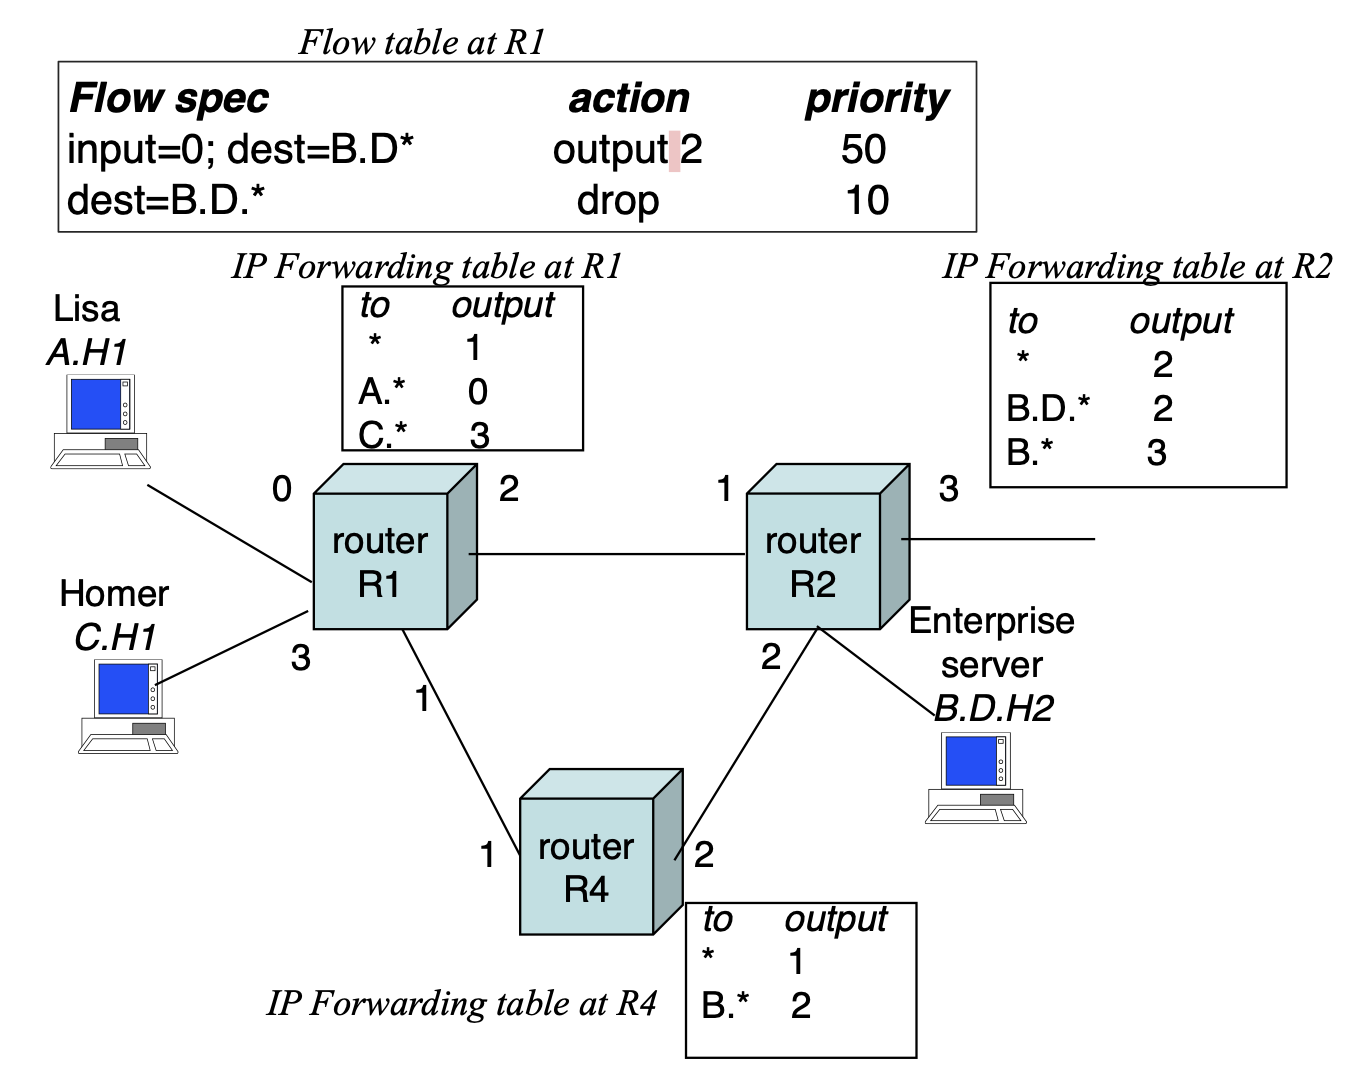
\includegraphics[width=0.7\textwidth]{images/sdns-question}
    \label{fig:LABEL}
\end{figure}

\vspace{0.3cm}

A. Lisa: 1, Homer: 1 \\
B. Lisa: 1, Homer: 2 \\
C. Lisa: 2, Homer: 1 \\
D. Lisa: 2, Homer : 2 \\
E. None of the above
F. I don't know \\

\textbf{Answer:} E \\

Packets from Lisa to enterprise server match the two flow rules; Packets from Homer to enterprise server match the second flow rule and are dropped by R1. 
\end{tcolorbox}


\subsection*{Software Defined Networks (SDN) in practice}

\begin{minipage}{0.5\textwidth}
\textcolor{red}{What?} A central \textcolor{blue}{\textit{controller}} application manages the flow tables in routers and/or switches

\textcolor{red}{How?}
\begin{itemize}
	\item The central controller decides rules and communicates them to local controllers on routers/switches
	\item Local controllers, called "\textcolor{red}{\textit{listeners}}", write the flow tables on routers or switches
	\item Protocol between local controller and central controller is e.g., OpenFlow, over TCP connections
\end{itemize}

\textcolor{red}{Where?} Mainly in large data centers, also for 5G cellular.
\end{minipage}
\hfill
\begin{minipage}{0.5\textwidth}
\centering
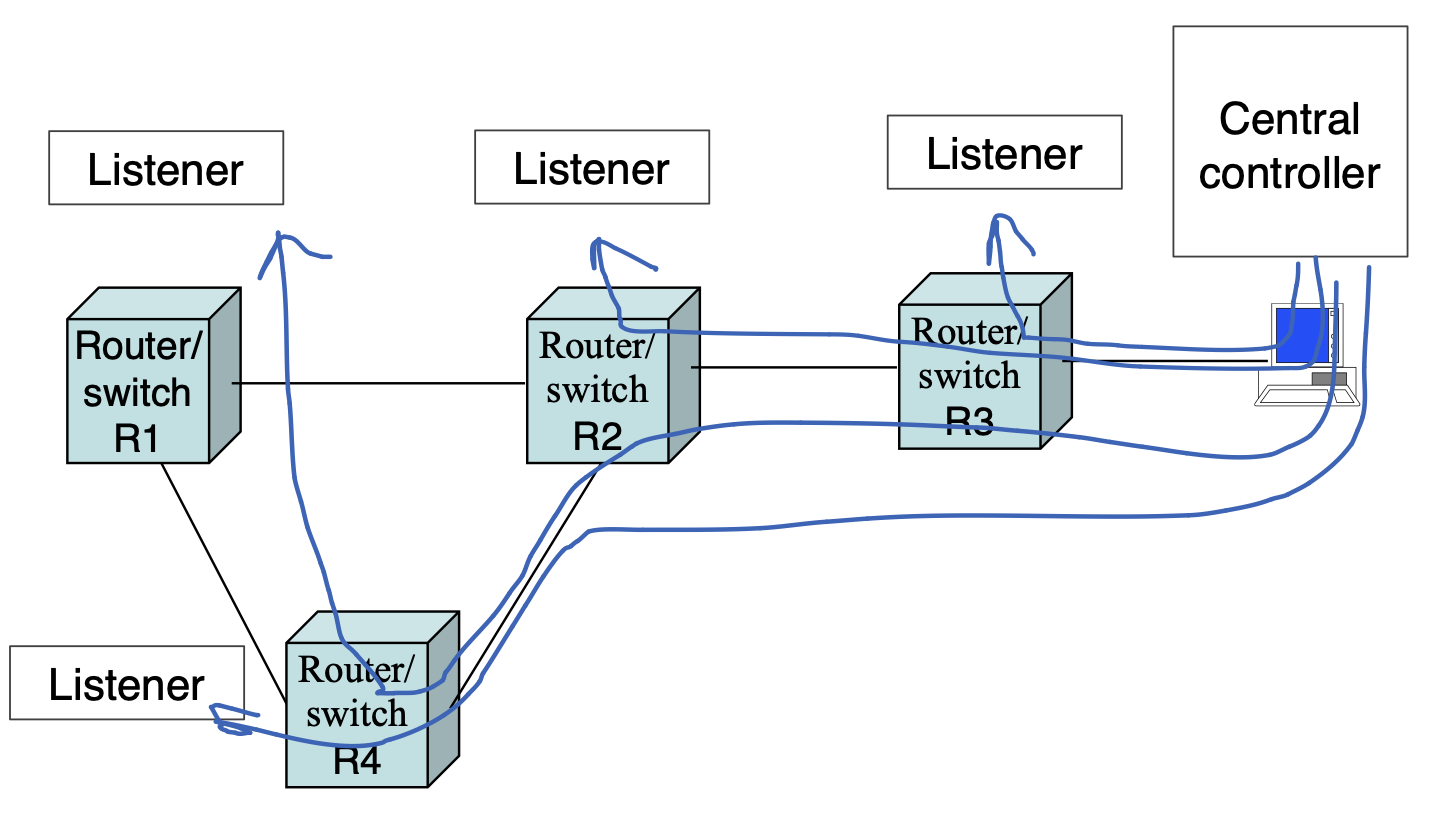
\includegraphics[width=\linewidth]{images/sdns}
\end{minipage}


\begin{tcolorbox}[
  colback=gray!15,     % background color
  colframe=black!50,    % border color
  boxrule=1pt,       % border thickness
  arc=3mm,             % rounded corners
  left=4mm, right=4mm, top=2mm, bottom=2mm % padding
]
\textbf{Do we need OSPF (or another routing protocol) if we have SDN ?}
% Quick centered image
\begin{figure}[H]
    \centering
    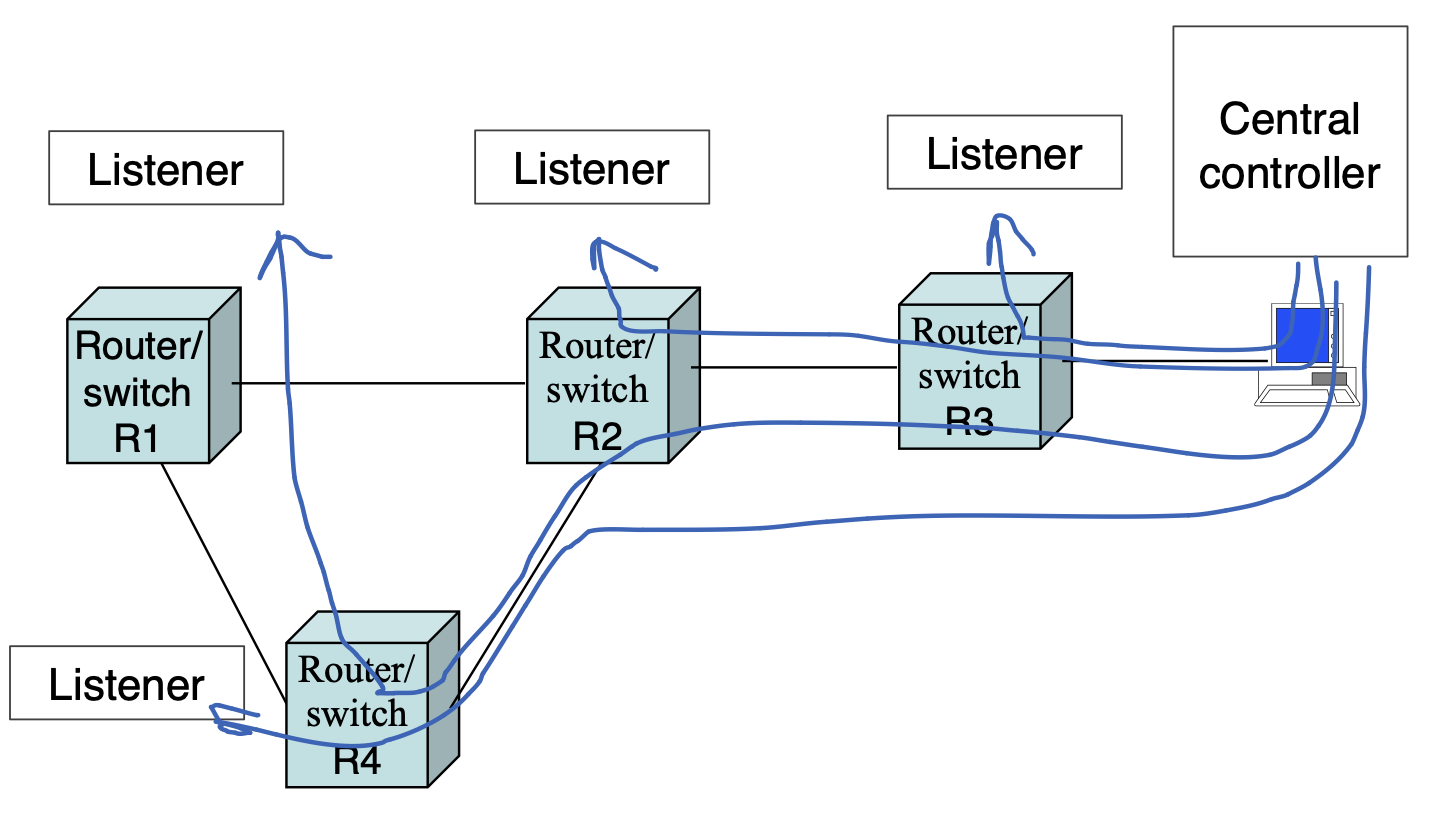
\includegraphics[width=0.6\textwidth]{images/sdns}
    \label{fig:LABEL}
\end{figure}

\vspace{0.3cm}
A. No because flow tables can replace IP forwarding tables \\
B. Yes because flow tables cannot replace IP forwarding tables \\
C. Yes because the central controller needs a way to communicate with local controllers \\
D. I don't know \\

\textbf{Answer:} C. \\
The central controller communicates with the local controllers in routers over TCP connections. This needs that IP forwarding tables are functional, which (in principle) requires OSPF or some other routing protocol. \\

But this common-sense observation may not always hold. Remember the \textcolor{blue}{\textit{Facebook outage of Oct 4, 2021}}, where it seems that routers were disconnected remotely and it was impossible to bring them back in.  
\end{tcolorbox}

\section*{Conclusion}
Routing protocol automatically build connectivity and repair failures. 

With link state routing (like OSPF): 
\begin{itemize}
	\item All routers compute their own link state database, replicated in all routers
	\item All routers compute their routing tables using Dijkstra and the link state database
	\item Convergence after failure is fast (if detection is fast)
	\item Non-standard cost definitions are possible; can be used for routing specific flows in different ways
	\item Large domains must be split into areas
\end{itemize}

More control can be obtained by an outside application (SDN) at the expense of losing the robustness of distributed protocols. SDN is used today primarily with switches, but also with routers in some networks.
\end{document}
